\documentclass[border=3pt]{standalone}

% Drawing
\usepackage{tikz}

% Tikz Library
\usetikzlibrary{angles, quotes, shapes, decorations.markings, calc, arrows.meta}

% Styles
%% Left and Bottom Right Rays' Style
\tikzset{ray/.style = {postaction=decorate,decoration={markings,
						 mark=at position .52 with \arrow{stealth},
						 mark=between positions 0.1 and 0.4 step 0.5cm with with{
						 \draw[fill=red, draw=red] circle [radius=1pt];
						 \draw[red, {Latex[length=1.3mm, width=1.5mm]}-{Latex[length=1.3mm, width=1.5mm]}] (0,-7pt) -- (0,7pt);},
						 mark=between positions 0.6 and 0.9 step 0.5cm with with{\draw[fill=red, draw = red] circle[radius=1pt];
						 \draw[red, {Latex[length=1.3mm, width=1.5mm]}-{Latex[length=1.3mm, width=1.5mm]}] (0,-7pt) -- (0,7pt);},
						 								}
						 }
		}
% Upper Right Ray Style
\tikzset{polray/.style = {postaction=decorate,decoration={markings,
						 mark=at position .52 with \arrow{stealth},
						 mark=between positions 0.1 and 0.4 step 0.5cm with with{\draw[fill=red, draw=red] circle [radius=1pt];},
						 mark=between positions 0.6 and 0.9 step 0.5cm with with{\draw[fill=red, draw = red] circle[radius=1pt];}						 			}
						 }
		}

% Notation
\usepackage{amsmath}

\begin{document}
	
% Right Angle Mark
\def\MarkRightAngle[size=#1](#2,#3,#4){\draw[thick] ($(#3)!#1!(#2)$) -- ($($(#3)!#1!(#2)$)!#1!90:(#2)$) -- ($(#3)!#1!(#4)$)}

	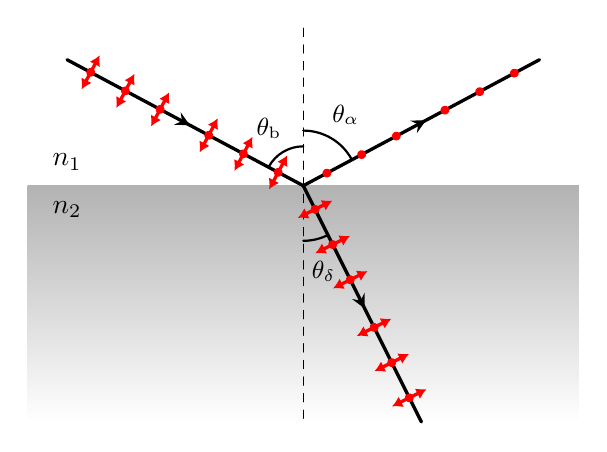
\begin{tikzpicture}[line cap=round, line join=round]
%		% Grid
%		\draw[dotted, black!20] (0,0) grid (8,8);
%		
%		\node at (-2ex,-2ex) {$0$};
%		\foreach \i in {1,...,8}
%		{
%			\node at (-2ex,\i) {$\i$};
%			\node at (\i,-2ex) {$\i$};
%		}
		
		% Coordinates
		\coordinate (A) at (4,5);
		\coordinate (B) at (4,0);
		
		\coordinate (a) at (1,4.6);
		\coordinate (C) at (4,3);
		\coordinate (a') at (7,4.6);
		\coordinate (b) at (5.5,0);
		
		% Second Material
		\node[rectangle, top color=black!30, bottom color=white, minimum width=7cm, minimum height=3cm] at (4,1.5) {};
		
		\draw[dashed] (A) -- (B);
		
		% Rays
		\draw[very thick, ray] (a) -- (C);
		\draw[very thick, polray] (C) -- (a');
		\draw[very thick, ray] (C) -- (b);
		
		% Angles
		\MarkRightAngle[size=6pt](b,C,a');
		%
		\pic[draw, thick, "\small$\theta_\text{b}$", angle radius = 0.5cm, angle eccentricity = 1.7pt] {angle = A--C--a};
		%
		\pic[draw, thick, "\small$\theta_\alpha$", angle radius = 0.7cm, angle eccentricity = 1.5pt] {angle = a'--C--A};
		%
		\pic[draw, thick, "\small$\theta_\delta$", angle radius = 0.7cm, angle eccentricity = 1.6pt] {angle = B--C--b};
		
		% Text Nodes
		\node at (1,3.3) {$n_1$};
		\node at (1,2.7) {$n_2$};
	\end{tikzpicture}
	
\end{document}